%% Included in decks: design-handbook
\setSlideVersion{1-0-0}
\begin{standardframe}{Widgets: containers and choices}
\begin{columns}[T,onlytextwidth]
\begin{column}{.48\linewidth}
\textbf{Light}\par
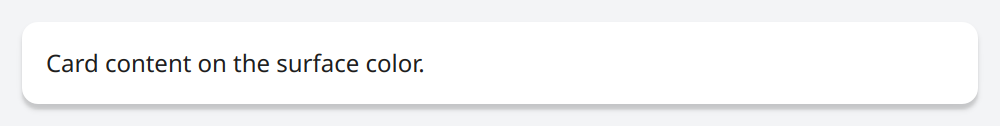
\includegraphics[width=\linewidth,height=0.11\textheight,keepaspectratio]{media/card-light.png}\par\smallskip
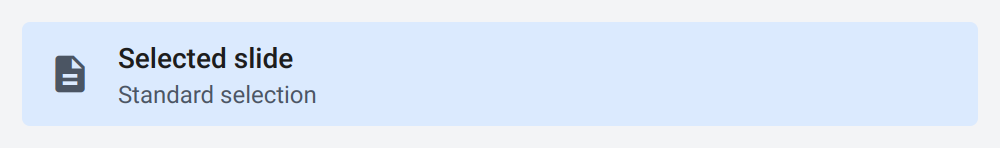
\includegraphics[width=\linewidth,height=0.11\textheight,keepaspectratio]{media/row-button-light.png}\par\smallskip
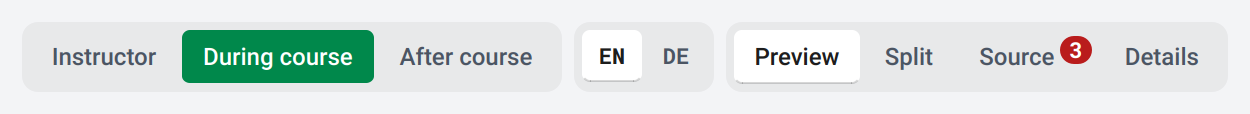
\includegraphics[width=\linewidth,height=0.11\textheight,keepaspectratio]{media/segmented-control-light.png}\par\smallskip
\end{column}
\begin{column}{.48\linewidth}
\textbf{Dark}\par
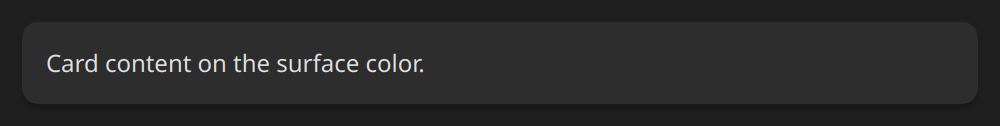
\includegraphics[width=\linewidth,height=0.11\textheight,keepaspectratio]{media/card-dark.png}\par\smallskip
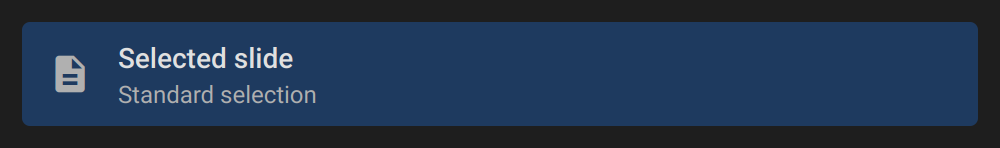
\includegraphics[width=\linewidth,height=0.11\textheight,keepaspectratio]{media/row-button-dark.png}\par\smallskip
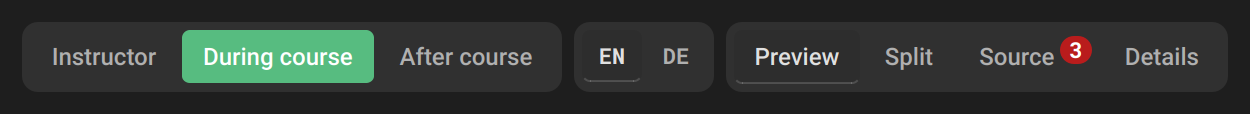
\includegraphics[width=\linewidth,height=0.11\textheight,keepaspectratio]{media/segmented-control-dark.png}\par\smallskip
\end{column}
\end{columns}
\begin{itemize}
\item Card: group related content. RowButton: choose an item, with standard blue selection.
\item SegmentedControl: switch among a small set of peer views.
\end{itemize}
\end{standardframe}
